\hypertarget{vandeWiel_8c}{
\section{vandeWiel.c File Reference}
\label{vandeWiel_8c}\index{vandeWiel.c@{vandeWiel.c}}
}
{\tt \#include $<$R.h$>$}\par
{\tt \#include $<$Rmath.h$>$}\par
{\tt \#include $<$Rdefines.h$>$}\par


Include dependency graph for vandeWiel.c:\nopagebreak
\begin{figure}[H]
\begin{center}
\leavevmode
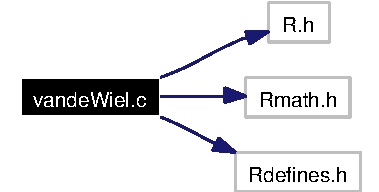
\includegraphics[width=118pt]{vandeWiel_8c__incl}
\end{center}
\end{figure}
\subsection*{Classes}
\begin{CompactItemize}
\item 
struct \hyperlink{structcelW}{celW}
\end{CompactItemize}
\subsection*{Functions}
\begin{CompactItemize}
\item 
double \hyperlink{vandeWiel_8c_dd09844ac40346e216f503f95e644970}{binomi} (int m, int n)
\item 
\hyperlink{structcelW}{celW} $\ast$$\ast$ \hyperlink{vandeWiel_8c_03d7f636d17008a6fbe230458a92ddba}{reserveW} (int a, int b)
\item 
void \hyperlink{vandeWiel_8c_f72cc4501998ae01067d5555382b1609}{FreeW} (int a, \hyperlink{structcelW}{celW} $\ast$$\ast$W)
\item 
void \hyperlink{vandeWiel_8c_402c3e72a2fa3d600d4a4e8ace9f040b}{initW} (int a, int b, \hyperlink{structcelW}{celW} $\ast$$\ast$W)
\item 
void \hyperlink{vandeWiel_8c_e1d7e7e209f5b99745c8bca03057f761}{mult} (\hyperlink{structcelW}{celW} $\ast$tem, int a, int b, int rank, double $\ast$rs)
\item 
void \hyperlink{vandeWiel_8c_965c6db84dd8be42e1313d8c3ef9a784}{plus} (\hyperlink{structcelW}{celW} $\ast$$\ast$W, \hyperlink{structcelW}{celW} $\ast$tempie, int a, int b)
\item 
void \hyperlink{vandeWiel_8c_2f117e88849518e50d7d0eef3af07bf0}{mymergesort} (\hyperlink{structcelW}{celW} temptw, long tijd)
\item 
void \hyperlink{vandeWiel_8c_59f513c0ee260be89ad37daacf49e7e8}{fillcell} (\hyperlink{structcelW}{celW} $\ast$$\ast$W, int i1, int j1, int r, double $\ast$rs)
\item 
void \hyperlink{vandeWiel_8c_d0195ffa22342dfadee0abeb564931dc}{mirrorW} (\hyperlink{structcelW}{celW} $\ast$$\ast$W, int ce, int bep, int start, double $\ast$rs)
\item 
void \hyperlink{vandeWiel_8c_fb521caca26031c6fa9e92450685f5d1}{makeW} (\hyperlink{structcelW}{celW} $\ast$$\ast$W, int a, int b, int start, double $\ast$rs)
\item 
void \hyperlink{vandeWiel_8c_76539410f65d0d4c5105bacf1b32f093}{cumulcoef} (\hyperlink{structcelW}{celW} $\ast$$\ast$W, int i1, int j1)
\item 
double \hyperlink{vandeWiel_8c_14307006f6d9ec07bdfce7e853665bc5}{numbersmall} (int c, int b, double ob, \hyperlink{structcelW}{celW} $\ast$$\ast$W1, \hyperlink{structcelW}{celW} $\ast$$\ast$W2)
\item 
SEXP \hyperlink{vandeWiel_8c_a50657b564a35ab41b3e3e50e62c51b1}{R\_\-split\_\-up\_\-2sample} (SEXP scores, SEXP m, SEXP obs)
\end{CompactItemize}


\subsection{Detailed Description}
Exact Distribution of Two-Sample Permutation Tests van de Wiel split-up Algorithm

Author: Mark van de Wiel (2001-2005) $<$\href{mailto:m.a.v.d.wiel@TUE.nl}{\tt m.a.v.d.wiel@TUE.nl}$>$ with modifications for R by Torsten Hothorn $<$\href{mailto:Torsten.Hothorn@R-project.org}{\tt Torsten.Hothorn@R-project.org}$>$

\begin{Desc}
\item[Author:]\begin{Desc}
\item[Author]\end{Desc}
\end{Desc}
\begin{Desc}
\item[Date:]\begin{Desc}
\item[Date]\end{Desc}
\end{Desc}


Definition in file \hyperlink{vandeWiel_8c-source}{vandeWiel.c}.

\subsection{Function Documentation}
\hypertarget{vandeWiel_8c_dd09844ac40346e216f503f95e644970}{
\index{vandeWiel.c@{vandeWiel.c}!binomi@{binomi}}
\index{binomi@{binomi}!vandeWiel.c@{vandeWiel.c}}
\subsubsection{\setlength{\rightskip}{0pt plus 5cm}double binomi (int {\em m}, int {\em n})}}
\label{vandeWiel_8c_dd09844ac40346e216f503f95e644970}




Definition at line 37 of file vandeWiel.c.

Referenced by R\_\-split\_\-up\_\-2sample(), and reserveW().\hypertarget{vandeWiel_8c_76539410f65d0d4c5105bacf1b32f093}{
\index{vandeWiel.c@{vandeWiel.c}!cumulcoef@{cumulcoef}}
\index{cumulcoef@{cumulcoef}!vandeWiel.c@{vandeWiel.c}}
\subsubsection{\setlength{\rightskip}{0pt plus 5cm}void cumulcoef ({\bf celW} $\ast$$\ast$ {\em W}, int {\em i1}, int {\em j1})}}
\label{vandeWiel_8c_76539410f65d0d4c5105bacf1b32f093}




Definition at line 316 of file vandeWiel.c.

References celW::c, and celW::length.

Referenced by R\_\-split\_\-up\_\-2sample().\hypertarget{vandeWiel_8c_59f513c0ee260be89ad37daacf49e7e8}{
\index{vandeWiel.c@{vandeWiel.c}!fillcell@{fillcell}}
\index{fillcell@{fillcell}!vandeWiel.c@{vandeWiel.c}}
\subsubsection{\setlength{\rightskip}{0pt plus 5cm}void fillcell ({\bf celW} $\ast$$\ast$ {\em W}, int {\em i1}, int {\em j1}, int {\em r}, double $\ast$ {\em rs})}}
\label{vandeWiel_8c_59f513c0ee260be89ad37daacf49e7e8}




Definition at line 211 of file vandeWiel.c.

References celW::c, celW::length, mult(), mymergesort(), plus(), and celW::x.

Referenced by makeW().

Here is the call graph for this function:\nopagebreak
\begin{figure}[H]
\begin{center}
\leavevmode
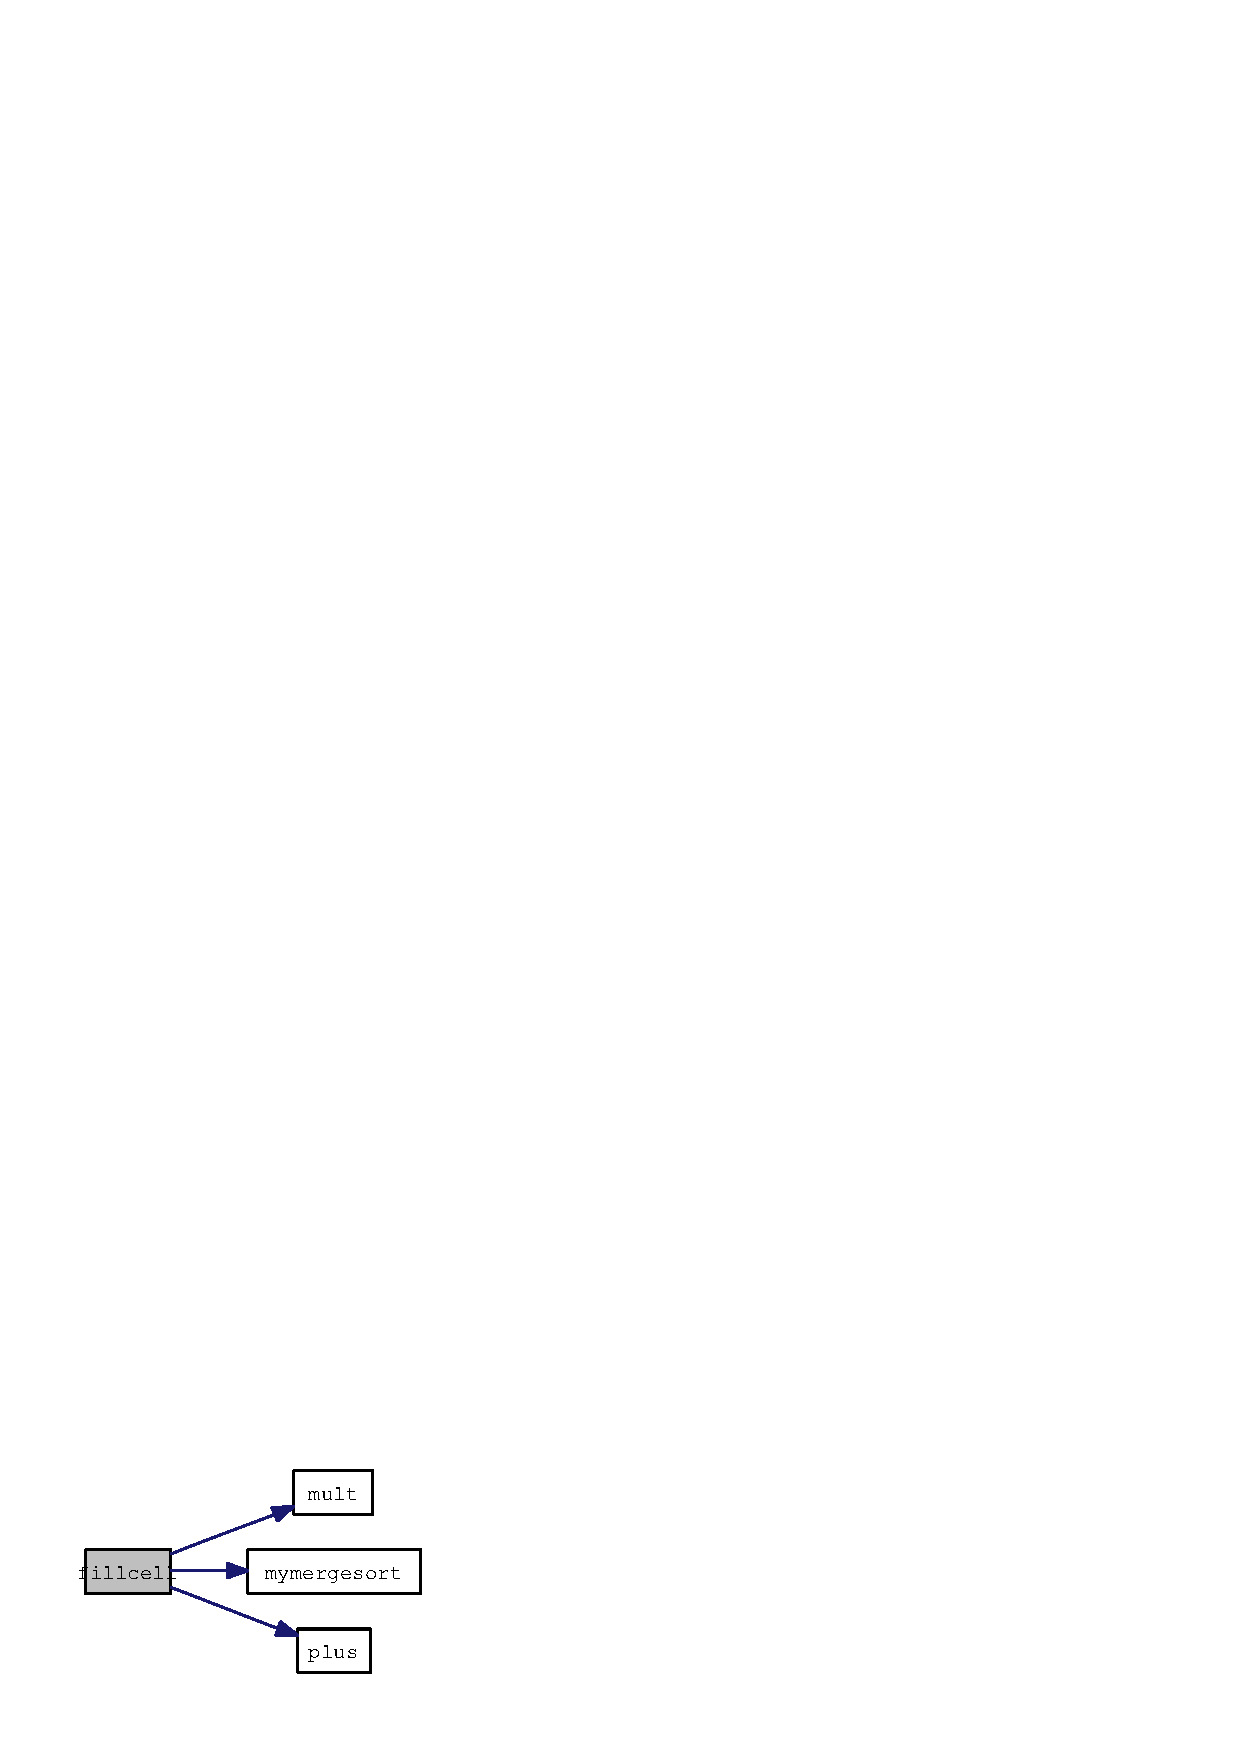
\includegraphics[width=103pt]{vandeWiel_8c_59f513c0ee260be89ad37daacf49e7e8_cgraph}
\end{center}
\end{figure}
\hypertarget{vandeWiel_8c_f72cc4501998ae01067d5555382b1609}{
\index{vandeWiel.c@{vandeWiel.c}!FreeW@{FreeW}}
\index{FreeW@{FreeW}!vandeWiel.c@{vandeWiel.c}}
\subsubsection{\setlength{\rightskip}{0pt plus 5cm}void FreeW (int {\em a}, {\bf celW} $\ast$$\ast$ {\em W})}}
\label{vandeWiel_8c_f72cc4501998ae01067d5555382b1609}




Definition at line 81 of file vandeWiel.c.

Referenced by R\_\-split\_\-up\_\-2sample().\hypertarget{vandeWiel_8c_402c3e72a2fa3d600d4a4e8ace9f040b}{
\index{vandeWiel.c@{vandeWiel.c}!initW@{initW}}
\index{initW@{initW}!vandeWiel.c@{vandeWiel.c}}
\subsubsection{\setlength{\rightskip}{0pt plus 5cm}void initW (int {\em a}, int {\em b}, {\bf celW} $\ast$$\ast$ {\em W})}}
\label{vandeWiel_8c_402c3e72a2fa3d600d4a4e8ace9f040b}




Definition at line 91 of file vandeWiel.c.

References celW::c, celW::length, and celW::x.

Referenced by R\_\-split\_\-up\_\-2sample().\hypertarget{vandeWiel_8c_fb521caca26031c6fa9e92450685f5d1}{
\index{vandeWiel.c@{vandeWiel.c}!makeW@{makeW}}
\index{makeW@{makeW}!vandeWiel.c@{vandeWiel.c}}
\subsubsection{\setlength{\rightskip}{0pt plus 5cm}void makeW ({\bf celW} $\ast$$\ast$ {\em W}, int {\em a}, int {\em b}, int {\em start}, double $\ast$ {\em rs})}}
\label{vandeWiel_8c_fb521caca26031c6fa9e92450685f5d1}




Definition at line 281 of file vandeWiel.c.

References fillcell(), and mirrorW().

Referenced by R\_\-split\_\-up\_\-2sample().

Here is the call graph for this function:\nopagebreak
\begin{figure}[H]
\begin{center}
\leavevmode
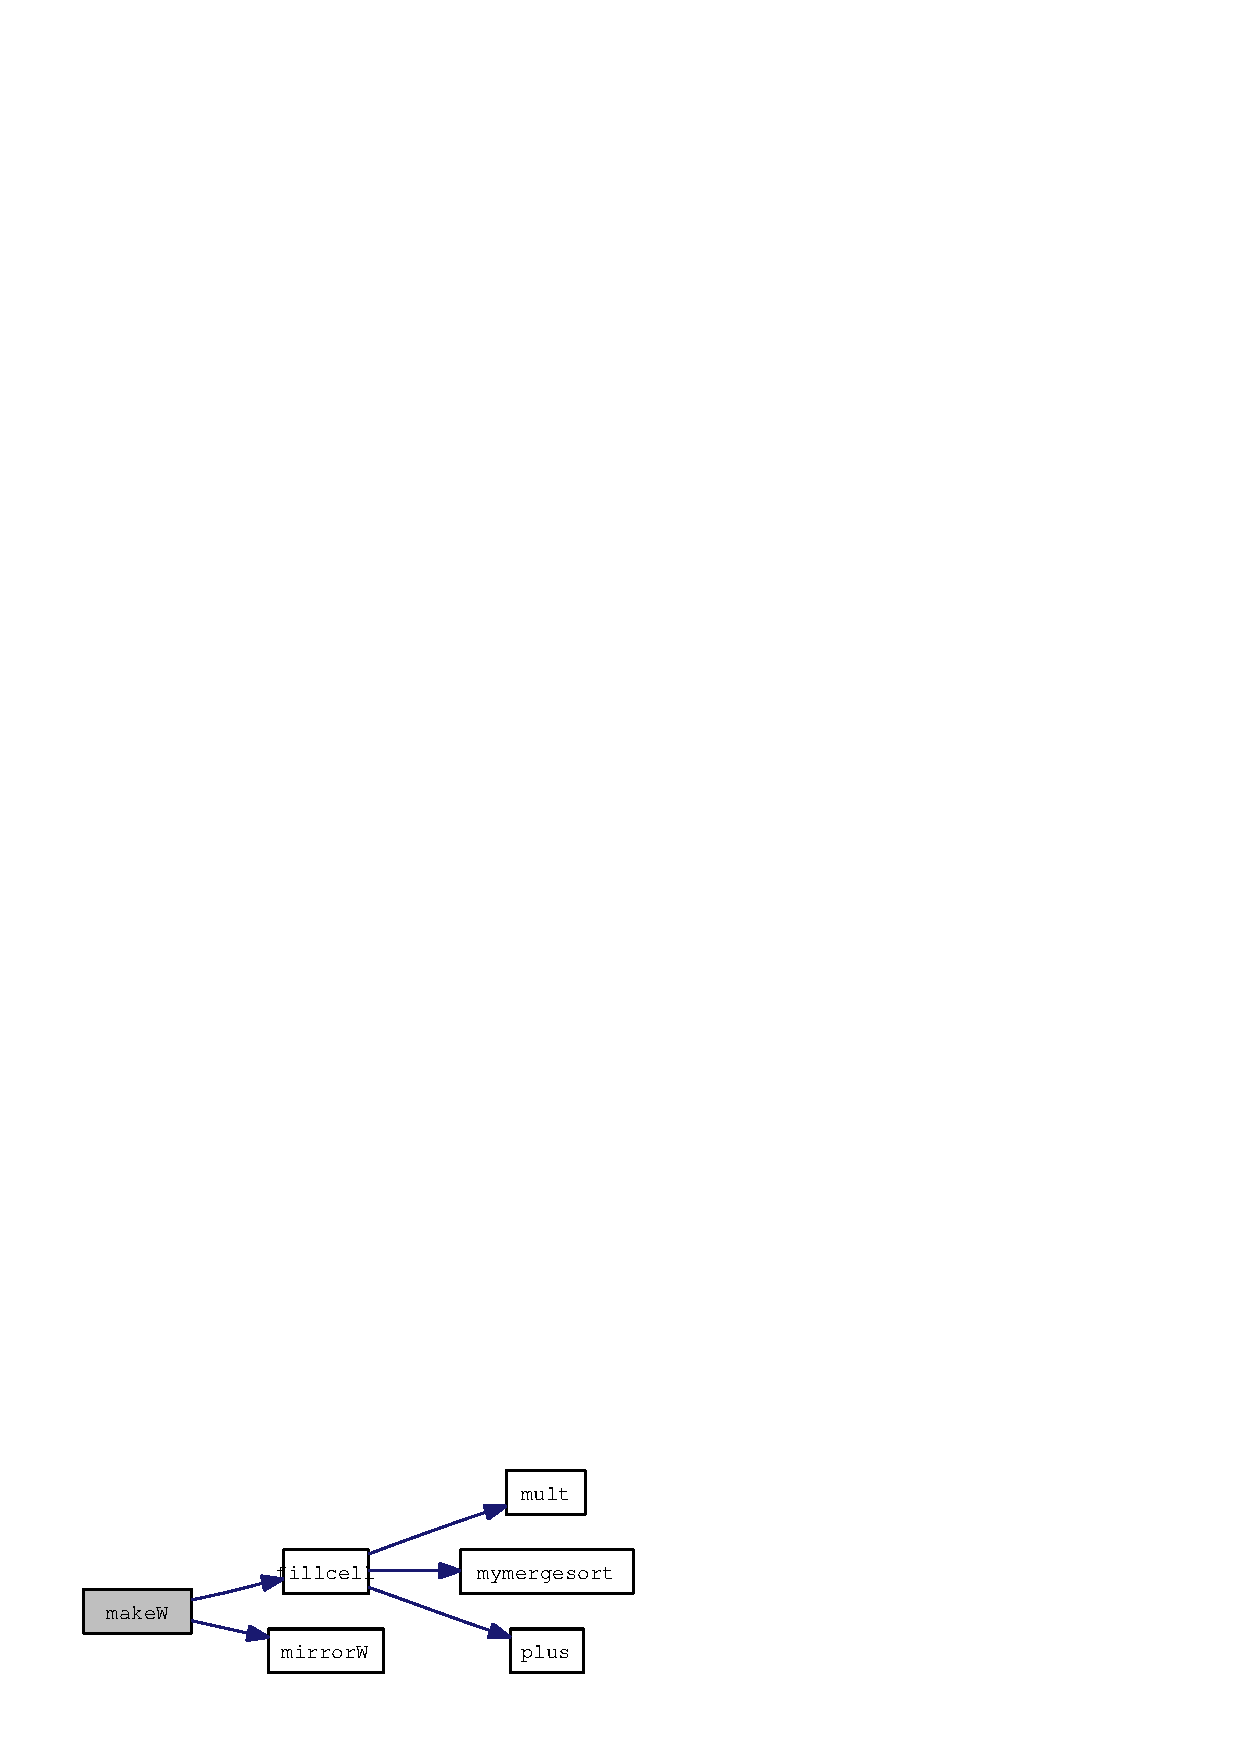
\includegraphics[width=154pt]{vandeWiel_8c_fb521caca26031c6fa9e92450685f5d1_cgraph}
\end{center}
\end{figure}
\hypertarget{vandeWiel_8c_d0195ffa22342dfadee0abeb564931dc}{
\index{vandeWiel.c@{vandeWiel.c}!mirrorW@{mirrorW}}
\index{mirrorW@{mirrorW}!vandeWiel.c@{vandeWiel.c}}
\subsubsection{\setlength{\rightskip}{0pt plus 5cm}void mirrorW ({\bf celW} $\ast$$\ast$ {\em W}, int {\em ce}, int {\em bep}, int {\em start}, double $\ast$ {\em rs})}}
\label{vandeWiel_8c_d0195ffa22342dfadee0abeb564931dc}




Definition at line 257 of file vandeWiel.c.

References celW::c, celW::length, and celW::x.

Referenced by makeW().\hypertarget{vandeWiel_8c_e1d7e7e209f5b99745c8bca03057f761}{
\index{vandeWiel.c@{vandeWiel.c}!mult@{mult}}
\index{mult@{mult}!vandeWiel.c@{vandeWiel.c}}
\subsubsection{\setlength{\rightskip}{0pt plus 5cm}void mult ({\bf celW} $\ast$ {\em tem}, int {\em a}, int {\em b}, int {\em rank}, double $\ast$ {\em rs})}}
\label{vandeWiel_8c_e1d7e7e209f5b99745c8bca03057f761}




Definition at line 106 of file vandeWiel.c.

References celW::length.

Referenced by fillcell().\hypertarget{vandeWiel_8c_2f117e88849518e50d7d0eef3af07bf0}{
\index{vandeWiel.c@{vandeWiel.c}!mymergesort@{mymergesort}}
\index{mymergesort@{mymergesort}!vandeWiel.c@{vandeWiel.c}}
\subsubsection{\setlength{\rightskip}{0pt plus 5cm}void mymergesort ({\bf celW} {\em temptw}, long {\em tijd})}}
\label{vandeWiel_8c_2f117e88849518e50d7d0eef3af07bf0}




Definition at line 159 of file vandeWiel.c.

References celW::c, celW::length, and celW::x.

Referenced by fillcell().\hypertarget{vandeWiel_8c_14307006f6d9ec07bdfce7e853665bc5}{
\index{vandeWiel.c@{vandeWiel.c}!numbersmall@{numbersmall}}
\index{numbersmall@{numbersmall}!vandeWiel.c@{vandeWiel.c}}
\subsubsection{\setlength{\rightskip}{0pt plus 5cm}double numbersmall (int {\em c}, int {\em b}, double {\em ob}, {\bf celW} $\ast$$\ast$ {\em W1}, {\bf celW} $\ast$$\ast$ {\em W2})}}
\label{vandeWiel_8c_14307006f6d9ec07bdfce7e853665bc5}




Definition at line 335 of file vandeWiel.c.

References celW::c, and celW::length.

Referenced by R\_\-split\_\-up\_\-2sample().\hypertarget{vandeWiel_8c_965c6db84dd8be42e1313d8c3ef9a784}{
\index{vandeWiel.c@{vandeWiel.c}!plus@{plus}}
\index{plus@{plus}!vandeWiel.c@{vandeWiel.c}}
\subsubsection{\setlength{\rightskip}{0pt plus 5cm}void plus ({\bf celW} $\ast$$\ast$ {\em W}, {\bf celW} $\ast$ {\em tempie}, int {\em a}, int {\em b})}}
\label{vandeWiel_8c_965c6db84dd8be42e1313d8c3ef9a784}




Definition at line 120 of file vandeWiel.c.

References celW::c, celW::length, and celW::x.

Referenced by fillcell().\hypertarget{vandeWiel_8c_a50657b564a35ab41b3e3e50e62c51b1}{
\index{vandeWiel.c@{vandeWiel.c}!R_split_up_2sample@{R\_\-split\_\-up\_\-2sample}}
\index{R_split_up_2sample@{R\_\-split\_\-up\_\-2sample}!vandeWiel.c@{vandeWiel.c}}
\subsubsection{\setlength{\rightskip}{0pt plus 5cm}SEXP R\_\-split\_\-up\_\-2sample (SEXP {\em scores}, SEXP {\em m}, SEXP {\em obs})}}
\label{vandeWiel_8c_a50657b564a35ab41b3e3e50e62c51b1}




Definition at line 375 of file vandeWiel.c.

References binomi(), cumulcoef(), FreeW(), initW(), makeW(), numbersmall(), and reserveW().

Here is the call graph for this function:\nopagebreak
\begin{figure}[H]
\begin{center}
\leavevmode
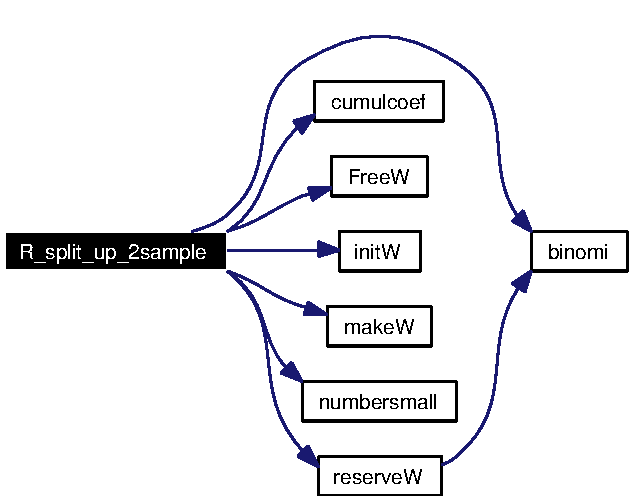
\includegraphics[width=241pt]{vandeWiel_8c_a50657b564a35ab41b3e3e50e62c51b1_cgraph}
\end{center}
\end{figure}
\hypertarget{vandeWiel_8c_03d7f636d17008a6fbe230458a92ddba}{
\index{vandeWiel.c@{vandeWiel.c}!reserveW@{reserveW}}
\index{reserveW@{reserveW}!vandeWiel.c@{vandeWiel.c}}
\subsubsection{\setlength{\rightskip}{0pt plus 5cm}{\bf celW}$\ast$$\ast$ reserveW (int {\em a}, int {\em b})}}
\label{vandeWiel_8c_03d7f636d17008a6fbe230458a92ddba}




Definition at line 51 of file vandeWiel.c.

References binomi(), celW::c, and celW::x.

Referenced by R\_\-split\_\-up\_\-2sample().

Here is the call graph for this function:\nopagebreak
\begin{figure}[H]
\begin{center}
\leavevmode
\includegraphics[width=95pt]{vandeWiel_8c_03d7f636d17008a6fbe230458a92ddba_cgraph}
\end{center}
\end{figure}
